\documentclass{standalone}
\usepackage{tikz}
\usepackage{ctex,siunitx}
\usepackage{tkz-euclide}
\usepackage{amsmath}
\usetikzlibrary{patterns, calc}
\usetikzlibrary {decorations.pathmorphing, decorations.pathreplacing, decorations.shapes,}
\begin{document}
\small
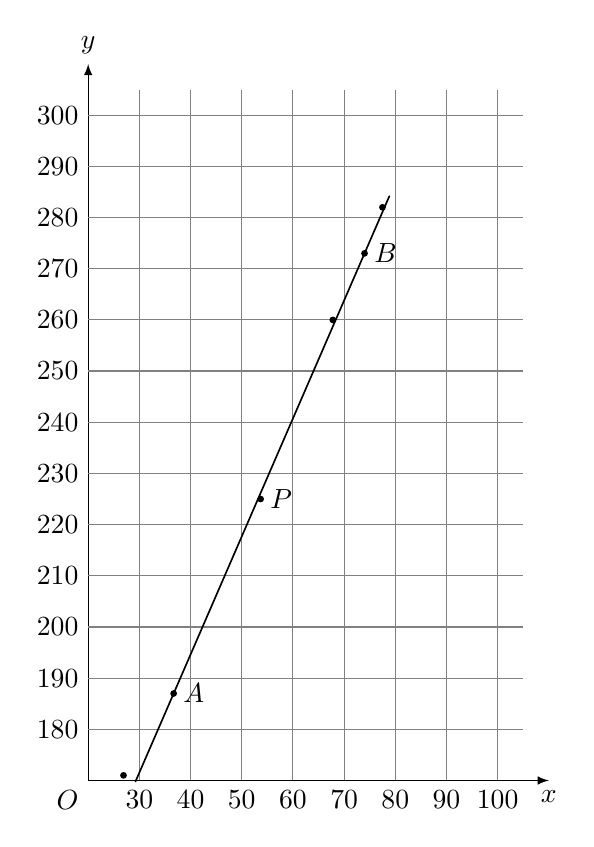
\begin{tikzpicture}[>=latex,scale=0.65]
  \draw[thin,->](0,0)--(9,0)node[below]{$x$};
  \draw[thin,->](0,0)--(0,14)node[above]{$y$};
  \tkzDefPoints{0/0/O,0.69/0.1/M,5.75/11.2/N,1.67/1.7/A,5.4/10.3/B,3.37/5.5/P,4.78/9/Q}
  \foreach \x[count=\i] in {30,40,...,100}
  {
    \draw[thin,gray](\i,0)--++(0,13.5)node[at start,below,text=black]{$\x$};
  }
  \foreach \x[count=\i] in {180,190,...,300}
  {
    \draw[thin,gray](0,\i)--++(8.5,0)node [at start,left,text=black]{$\x$};
  }
  \tkzDrawLine[semithick,add=0.2 and 0.13](A,B)
  \tkzDrawPoints[fill=black](M,N,A,B,P,Q)
  \tkzLabelPoints[right](A,B,P)
  \tkzLabelPoints[below left](O)
\end{tikzpicture}
\end{document}